\documentclass[11pt,a4paper, dvipdfmx]{jsarticle}
\usepackage{amsmath,amssymb}
\usepackage{amsthm}
\usepackage{ascmac}
\usepackage{bm}
\usepackage[dvipdfmx]{graphicx}	% required for `\includegraphics' (yatex added)
\usepackage{setspace}           % required for `\doublespace'
\usepackage{tikz}
\usepackage{tikz-cd}
\usetikzlibrary{angles, positioning, shapes, arrows.meta, decorations.pathmorphing}
%\usetikzlibrary{intersections, calc, arrows, positioning, arrows.meta}
\usepackage{tcolorbox}  % 定理環境の装飾
\tcbuselibrary{skins, breakable, theorems}
\usepackage{xcolor}
\usepackage{natbib}
\usepackage{pxrubrica}
\usepackage[margin=30truemm, left=40truemm, right=40truemm]{geometry}
\usepackage{thmbox}     % required for theorem environment with side bar
%
\setlength{\parskip}{3mm} %段落間にスペースを入れる


% \pagestyle{myheadings}
% \markright{\footnotesize \sf 2022秋期「哲学者のための数学」授業資料(大塚淳) \ \ 配布禁止}


\theoremstyle{definition}
\newtheorem[S]{exercise}{練習問題}[section]
\newtheorem[S]{example}{事例}[section]
\newtheorem[S]{fact}{事実}[section]
\newtheorem[S]{attn}{注意}[section]
\newtheorem[S]{develop}{発展}[section]
\renewcommand{\theattn}{}

\newtcbtheorem[auto counter, number within=section]{rei}{事例}{
    breakable,
    coltitle=black,
    fonttitle=\bfseries,
    enhanced, colback=white, frame hidden, borderline west = {0.5pt}{5pt}{black},
%    number freestyle={\noexpand\thesection.\noexpand\arabic{\tcbcounter}}
}{rei}

\newtcbtheorem[auto counter, number within=section]{prop}{命題}{
    breakable,
    coltitle=black,
    fonttitle=\bfseries,
    enhanced, colback=white, frame hidden, borderline west = {0.5pt}{5pt}{black},
%    number freestyle={\noexpand\thesection.\noexpand\arabic{\tcbcounter}}
}{prop}

\newtcbtheorem[number within=section]{renshu}{練習問題}{
    breakable,
    coltitle=black,
    fonttitle=\bfseries,
    enhanced, colback=white, frame hidden, borderline west = {0.5pt}{5pt}{black}
}{renshu}


\newtcbtheorem[number within=section]{hatten}{発展}{
    breakable,
    coltitle=black,
    fonttitle=\bfseries,
    enhanced, colback=white, frame hidden, borderline west = {0.5pt}{5pt}{black}
}{renshu}


\newtcbtheorem[number within=section]{dfn}{定義}{
    fonttitle=\bfseries,
    enhanced, colback=white
}{dfn}


% Bold face capital letters:
\newcommand{\bfzero}{\boldsymbol{0}}
\newcommand{\bfone}{\boldsymbol{1}}
\newcommand{\bfA}{\boldsymbol{A}}
\newcommand{\bfB}{\boldsymbol{B}}
\newcommand{\bfC}{\boldsymbol{C}}
\newcommand{\bfD}{\boldsymbol{D}}
\newcommand{\bfE}{\boldsymbol{E}}
\newcommand{\bfF}{\boldsymbol{F}}
\newcommand{\bfG}{\boldsymbol{G}}
\newcommand{\bfH}{\boldsymbol{H}}
\newcommand{\bfI}{\boldsymbol{I}}
\newcommand{\bfJ}{\boldsymbol{J}}
\newcommand{\bfK}{\boldsymbol{K}}
\newcommand{\bfL}{\boldsymbol{L}}
\newcommand{\bfM}{\boldsymbol{M}}
\newcommand{\bfN}{\boldsymbol{N}}
\newcommand{\bfO}{\boldsymbol{O}}
\newcommand{\bfP}{\boldsymbol{P}}
\newcommand{\bfQ}{\boldsymbol{Q}}
\newcommand{\bfR}{\boldsymbol{R}}
\newcommand{\bfS}{\boldsymbol{S}}
\newcommand{\bfT}{\boldsymbol{T}}
\newcommand{\bfU}{\boldsymbol{U}}
\newcommand{\bfV}{\boldsymbol{V}}
\newcommand{\bfW}{\boldsymbol{W}}
\newcommand{\bfX}{\boldsymbol{X}}
\newcommand{\bfY}{\boldsymbol{Y}}
\newcommand{\bfZ}{\boldsymbol{Z}}

\newcommand{\bfa}{\boldsymbol{a}}
\newcommand{\bfb}{\boldsymbol{b}}
\newcommand{\bfc}{\boldsymbol{c}}
\newcommand{\bfd}{\boldsymbol{d}}
\newcommand{\bfe}{\boldsymbol{e}}
\newcommand{\bff}{\boldsymbol{f}}
\newcommand{\bfk}{\boldsymbol{k}}
\newcommand{\bfm}{\boldsymbol{m}}
\newcommand{\bfn}{\boldsymbol{n}}
\newcommand{\bfo}{\boldsymbol{o}}
\newcommand{\bfp}{\boldsymbol{p}}
\newcommand{\bfq}{\boldsymbol{q}}
\newcommand{\bfr}{\boldsymbol{r}}
\newcommand{\bfs}{\boldsymbol{s}}
\newcommand{\bft}{\boldsymbol{t}}
\newcommand{\bfu}{\boldsymbol{u}}
\newcommand{\bfv}{\boldsymbol{v}}
\newcommand{\bfw}{\boldsymbol{w}}
\newcommand{\bfx}{\boldsymbol{x}}
\newcommand{\bfy}{\boldsymbol{y}}
\newcommand{\bfz}{\boldsymbol{z}}



% BB (???) capital letters:
\newcommand{\bbA}{\mathbb{A}}
\newcommand{\bbB}{\mathbb{B}}
\newcommand{\bbC}{\mathbb{C}}
\newcommand{\bbD}{\mathbb{D}}
\newcommand{\bbE}{\mathbb{E}}
\newcommand{\bbF}{\mathbb{F}}
\newcommand{\bbG}{\mathbb{G}}
\newcommand{\bbI}{\mathbb{I}}
\newcommand{\bbN}{\mathbb{N}}
\newcommand{\bbP}{\mathbb{P}}
\newcommand{\bbQ}{\mathbb{Q}}
\newcommand{\bbR}{\mathbb{R}}
\newcommand{\bbU}{\mathbb{U}}
\newcommand{\bbV}{\mathbb{V}}
\newcommand{\bbX}{\mathbb{X}}
\newcommand{\bbY}{\mathbb{Y}}
\newcommand{\bbZ}{\mathbb{Z}}
\newcommand{\bbone}{{\ifmmode\mathrm{1\!l}\else\mbox{\(\mathrm{1\!l}\)}\fi}}


% Caligraphic math capital letters:
\newcommand{\mcalA}{\mathcal{A}}
\newcommand{\mcalB}{\mathcal{B}}
\newcommand{\mcalC}{\mathcal{C}}
\newcommand{\mcalD}{\mathcal{D}}
\newcommand{\mcalE}{\mathcal{E}}
\newcommand{\mcalF}{\mathcal{F}}
\newcommand{\mcalG}{\mathcal{G}}
\newcommand{\mcalH}{\mathcal{H}}
\newcommand{\mcalI}{\mathcal{I}}
\newcommand{\mcalJ}{\mathcal{J}}
\newcommand{\mcalK}{\mathcal{K}}
\newcommand{\mcalL}{\mathcal{L}}
\newcommand{\mcalM}{\mathcal{M}}
\newcommand{\mcalN}{\mathcal{N}}
\newcommand{\mcalO}{\mathcal{O}}
\newcommand{\mcalP}{\mathcal{P}}
\newcommand{\mcalQ}{\mathcal{Q}}
\newcommand{\mcalS}{\mathcal{S}}
\newcommand{\mcalT}{\mathcal{T}}
\newcommand{\mcalU}{\mathcal{U}}
\newcommand{\mcalV}{\mathcal{V}}
\newcommand{\mcalX}{\mathcal{X}}
\newcommand{\mcalY}{\mathcal{Y}}
\newcommand{\mcalZ}{\mathcal{Z}}

% Graph nodes notations:
\newcommand{\PA}{\mathit{PA}}
\newcommand{\bfPA}{\mathbf{PA}}
\newcommand{\CH}{\mathit{CH}}
\newcommand{\bfCH}{\mathbf{CH}}
\newcommand{\DS}{\mathit{DS}}
\newcommand{\bfDS}{\mathbf{DS}}
\newcommand{\ND}{\mathit{ND}}
\newcommand{\bfND}{\mathbf{ND}}
\newcommand{\AN}{\mathit{an}}
\newcommand{\bfAN}{\mathbf{an}}
\newcommand{\pa}{\mathit{pa}}
\newcommand{\bfpa}{\mathbf{pa}}
\newcommand{\ch}{\mathit{ch}}
\newcommand{\bfch}{\mathbf{ch}}
\newcommand{\ds}{\mathit{ds}}
\newcommand{\bfds}{\mathbf{ds}}
\newcommand{\nd}{\mathit{nd}}
\newcommand{\bfnd}{\mathbf{nd}}
\newcommand{\an}{\mathit{an}}
\newcommand{\bfan}{\mathbf{an}}



\DeclareMathOperator*{\argmax}{arg\,max}
\DeclareMathOperator*{\argmin}{arg\,min}
\DeclareMathOperator*{\argsup}{arg\,sup}
\DeclareMathOperator*{\arginf}{arg\,inf}
\DeclareMathOperator{\erfc}{erfc}
\DeclareMathOperator{\diag}{diag}
\DeclareMathOperator{\cum}{cum}
\DeclareMathOperator{\sgn}{sgn}
\DeclareMathOperator{\tr}{tr}
\DeclareMathOperator{\spn}{span}
\DeclareMathOperator{\adj}{adj}
\DeclareMathOperator{\E}{\mathbb{E}}
\DeclareMathOperator{\var}{Var}
\DeclareMathOperator{\cov}{Cov}
\DeclareMathOperator{\corr}{corr}
\DeclareMathOperator{\sech}{sech}
\DeclareMathOperator{\sinc}{sinc}
\DeclareMathOperator*{\lms}{l.i.m.\,}
\newcommand{\varop}[1]{\var\left[{#1}\right]}
\newcommand{\covop}[2]{\cov\left({#1},{#2}\right)}
\newcommand{\T}{^\textrm{T}}
\newcommand\indep{\protect\mathpalette{\protect\independenT}{\perp}}
\def\independenT#1#2{\mathrel{\rlap{$#1#2$}\mkern2mu{#1#2}}}

\newcommand{\bfalpha}{\boldsymbol{\alpha}}
\newcommand{\bfbeta} {\boldsymbol{\beta}}
\newcommand{\bfgamma}{\boldsymbol{\gamma}}
\newcommand{\bfeta}  {\boldsymbol{\eta}}
\newcommand{\bftheta}{\boldsymbol{\theta}}
\newcommand{\bflambda}   {\boldsymbol{\lambda}}
\newcommand{\bfmu}   {\boldsymbol{\mu}}
\newcommand{\bfnu}   {\boldsymbol{\nu}}
\newcommand{\bfxi}   {\boldsymbol{\xi}}
\newcommand{\bfpsi}  {\boldsymbol{\psi}}
\newcommand{\bfphi}   {\boldsymbol{\phi}}
\newcommand{\bfrho}   {\boldsymbol{\rho}}
\newcommand{\bfvarepsilon}{\boldsymbol{\varepsilon}}
%\newcommand{\qed}{{qed}}
%\newcommand{\eqalignno}[1]{\begin{array}{ccccccc}#1\end{array}}

\newcommand{\bfGamma}{\boldsymbol{\Gamma}}
\newcommand{\bfTheta}{\boldsymbol{\Theta}}
\newcommand{\bfLambda}   {\boldsymbol{\Lambda}}
\newcommand{\bfPsi}  {\boldsymbol{\Psi}}
\newcommand{\bfPhi}   {\boldsymbol{\Phi}}
\newcommand{\bfSigma}  {\boldsymbol{\Sigma}}
\newcommand{\bfOmega}  {\boldsymbol{\Omega}}


% DISTRIBUTIOoNS: 
\newcommand{\normal}{\mathcal{N}}
\newcommand{\binomial}{\mathcal{B}}
\newcommand{\multinomial}{\mathcal{M}}
\newcommand{\exponential}{\mathcal{E}}
\newcommand{\geometric}{\mathcal{G}}
\newcommand{\poisson}{\mbox{Poisson}}
\newcommand{\uniform}{\mbox{Uniform}}

% Logic
\newcommand{\true}{\texttt{true}}
\newcommand{\false}{\texttt{false}}


%PSTricks (commande for latent nodes)
\newcommand{\lnode}[4]{ \cnode(#1){#2}{#3}\rput(#1){\footnotesize#4} }

% KEEPING TRACK OF WORK
\newcommand{\todo}[1]
{
{\color{red}{
[TODO: #1]}}
\addcontentsline{toc}{subsection}{TO DO: #1}
}

\newcommand{\fixme}[1]{{\color{red}{#1}}}

\newenvironment{answer}[1]
{\par \color{blue}{#1}}
{}


\newcommand{\note}[2]
{
{\color{red}{
[#1: #2]}}
}




\makeatletter
% define \citepos for posesive citation (e.g. Otsuka's (2015))
\DeclareRobustCommand\citepos
  {\begingroup
   \let\NAT@nmfmt\NAT@posfmt% ...except with a different name format
   \NAT@swafalse\let\NAT@ctype\z@\NAT@partrue
   \@ifstar{\NAT@fulltrue\NAT@citetp}{\NAT@fullfalse\NAT@citetp}}

\let\NAT@orig@nmfmt\NAT@nmfmt
\def\NAT@posfmt#1{\NAT@orig@nmfmt{#1's}}
\makeatother




% Code for drawing color circle used in topology (pathconnectedness)
\usepackage{xparse}
\ExplSyntaxOn

\keys_define:nn { colour_transition_circle } {
    inner   .fp_set:N   = \l__inner_radius,
    inner   .initial:n  = {2},
    outer   .fp_set:N   = \l__outer_radius,
    outer   .initial:n  = {3},
    angle   .fp_set:N   = \l__start_angle,
    angle   .initial:n  = {0}
}

\NewDocumentCommand \ColourTransitionCircle { O{} m } {
\group_begin:
    \keys_set:nn { colour_transition_circle } {#1}
    \clist_clear:N \l_tmpa_clist
    \clist_map_inline:nn {#2} {
        \clist_put_right:Nn \l_tmpa_clist {##1}
        %\clist_put_right:Nn \l_tmpa_clist {##1}
    }
    \exp_args:Nx \col_trans_circ:n \l_tmpa_clist
\group_end:
}

\cs_new_protected:Npn \col_trans_circ:n #1 {
    \int_step_inline:nnnn {1} {1} {\clist_count:n {#1} - 1} {
        \path[top~color=\clist_item:nn {#1} {##1}, bottom~color=\clist_item:nn {#1} {##1+1}, shading~angle={270-(180-360/\clist_count:n {#1})/2+(##1-1)*360/\clist_count:n {#1}+\fp_use:N \l__start_angle}] ({\fp_use:N \l__inner_radius*cos((##1-1)*360/\clist_count:n {#1}+\fp_use:N \l__start_angle)},{\fp_use:N \l__inner_radius*sin((##1-1)*360/\clist_count:n {#1}+\fp_use:N \l__start_angle)}) arc[radius = \fp_use:N \l__inner_radius, start~angle={(##1-1)*360/\clist_count:n {#1}+\fp_use:N \l__start_angle}, delta~angle=360/\clist_count:n {#1}] -- ({\fp_use:N \l__outer_radius*cos(##1*360/\clist_count:n {#1}+\fp_use:N \l__start_angle)},{\fp_use:N \l__outer_radius*sin(##1*360/\clist_count:n {#1}+\fp_use:N \l__start_angle)}) arc[radius = \fp_use:N \l__outer_radius, start~angle={##1*360/\clist_count:n {#1}+\fp_use:N \l__start_angle}, delta~angle=-360/\clist_count:n {#1}] -- cycle;
    }
    \path[top~color=\clist_item:nn {#1} {\clist_count:n {#1}}, bottom~color=\clist_item:nn {#1} {1}, shading~angle={180-180/\clist_count:n {#1}+\fp_use:N \l__start_angle}]({\fp_use:N \l__inner_radius*cos((\clist_count:n {#1}-1)*360/\clist_count:n {#1}+\fp_use:N \l__start_angle)},{\fp_use:N \l__inner_radius*sin((\clist_count:n {#1}-1)*360/\clist_count:n {#1}+\fp_use:N \l__start_angle)}) arc[radius = \fp_use:N \l__inner_radius, start~angle={(\clist_count:n {#1}-1)*360/\clist_count:n {#1}+\fp_use:N \l__start_angle}, delta~angle=360/\clist_count:n {#1}] -- ({\fp_use:N \l__outer_radius*cos(\clist_count:n {#1}*360/\clist_count:n {#1}+\fp_use:N \l__start_angle)},{\fp_use:N \l__outer_radius*sin(\clist_count:n {#1}*360/\clist_count:n {#1}+\fp_use:N \l__start_angle)}) arc[radius = \fp_use:N \l__outer_radius, start~angle={\clist_count:n {#1}*360/\clist_count:n {#1}+\fp_use:N \l__start_angle}, delta~angle=-360/\clist_count:n {#1}] -- cycle;
}

\ExplSyntaxOff

\begin{document}


\title{4. 束とブール代数}
\author{2025秋期「哲学者のための数学」授業資料(大塚淳)}
\date{ver. \today}
\maketitle

\section{関係から代数へ}
我々は前章で,一定の公理を満たす二項関係を備えた集合として,順序構造を定義した.
順序は整数$\bbN$や実数$\bbR$など,様々な数学的集合が持つ基本的な構造でもある.
しかし順序だけでは,数の構造は組み尽くせていない.
なんとなれば,数は単に順序付けられているだけでなく,その中で足し算や掛け算などの演算が定義されているからだ.
そうした演算が定義された数学的構造を,一般に\emph{代数}(algebra)という.
この章では,そうした代数のプリミティブな形として,\emph{束}(lattice),およびその延長線上に定義される\emph{ブール代数}(boolean algebra)を紹介する.
実は束自体,順序構造の延長線上にあるもので,この意味で本章で扱う対象はすべて半順序でもある.

ブール代数は,とりわけ論理学との関係において非常に重要である.
後述するブール代数の演算子である「交わり」$\wedge$と「結び」$\vee$は,その見た目通り論理学における「かつ」と「または」に対応し,全体として論理計算の代数的構造を示している.
またそれ以外にも,本章で見るように,束は我々の「概念」が持つ階層的構造をモデル化するのにも用いることができる.
このように束は,言ってみれば「順序に毛が生えたもの」に過ぎないにもかかわらず,様々な可能性を持ち,突き詰めると奥が深い.
その本章では,その一部を概観してみよう.

\section{束}

まず,半順序とは反射的($x \preceq x$),反対称的($x \preceq y$かつ$y \preceq x$なら$x=y$),推移的($x \preceq y, y \preceq z$なら$x \preceq z$)な関係であったことを思い起こそう.
さらに前章で,順序の部分集合$A$のどれよりも大きい元たちのなかで一番小さい「スレスレの上界」として上限(およびその逆の「スレスレの下界」として下限)を定めた.
\emph{束}(lattice)とは,そうした上限・下限がどの元のペアにも存在するような半順序のことである.

\begin{dfn}{束}{lattice}
束とは半順序集合$\langle X, \preceq \rangle$であり,どの2元$x, y \in X$に対しても,上限および下限が存在するものである.
$x, y$の上限を\emph{結び}(join)といい,$x \vee y$で表す.またその下限を\emph{交わり}(meet)といい,$x \wedge y$で表す.

一般に束は三つ組$\langle X, \vee, \wedge \rangle$で表されるが,誤解のないときは単に束$X$と表す.
\end{dfn}

なんてことはない,これだけである.
束の定義は,単にどの元$x, y$に対してもその上限と下限があって,それらをそれぞれ$x \vee x$および$x \wedge y$という表記で表すことにする,と言っているに過ぎない.
しかし見方を変えると,この条件を束上の\emph{演算}の定義として捉えることができる.
つまり$\vee$を「2つの元の結びをとる演算」,$x \vee y$を「$x$と$y$に演算$\vee$を施した結果」として見るのである.
言い換えれば,$\vee, \wedge$を次のような2項関数として見るということである.
\begin{align*}
 \vee: X \times X \to X &, \ \ \ (x, y) \mapsto x \vee y \\
 \wedge: X \times X \to X &, \ \ \ (x, y) \mapsto x \wedge y 
\end{align*}
これは,例えば足し算「+」が二つの数$(n, m)$から別の数$n + m$への2項関数であるのと同様である.
そして上の束の定義は,こうした演算が\emph{閉じている}(closed),つまりどのような二元に適用しても,これらの演算を行った結果がちゃんと同じ束の中に含まれている,ということを保証している.
かくして我々は,最初の代数的演算を手に入れた.

半順序同様,束もハッセ図によって図示することができる.
図\ref{fig:lattice}の左側は束の一例である.
実際,すべてのペアについて,その上限・下限が一意に定まっている.
上の演算を確認すると,例えば$b\vee d = e$であり,$c \wedge f = a$である.
一方,右側のハッセ図は半順序であるが束ではない.
というのも,ペア$(b, c)$は上界として$d, e, f$を持つが,$d$の$e$の間には大小関係がないので,最小かは定まらない,つまり上限がないからだ.同様に$(d, e)$は下限を持たない.
よって演算$b \vee c, d \wedge e$が一意に定義されず,束の条件を満たさない.
\begin{figure}[h]
    \centering
    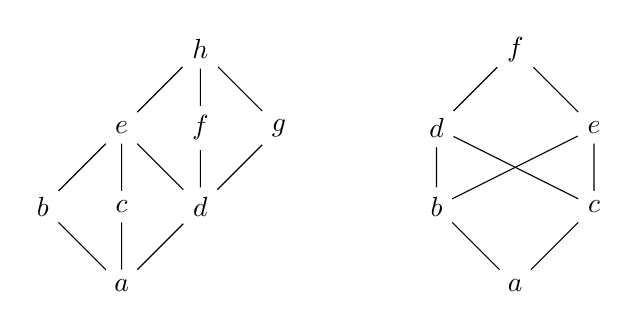
\begin{tikzpicture}[node distance=1.5cm]
        \begin{scope}
            \node (a) at (0,0) {$a$};
            \node (b) at (-1,1) {$b$};
            \node (c) at (0,1) {$c$};
            \node (d) at (1,1) {$d$};
            \node (e) at (0,2) {$e$};
            \node (f) at (1,2) {$f$};
            \node (g) at (2,2) {$g$};
            \node (h) at (1,3) {$h$};
            \draw (a)--(b)--(e)--(h)--(f)--(d)--(e)--(c)--(a)--(d)--(g)--(h);
        \end{scope}
        \begin{scope}[xshift=5cm]
            \node (a) at (0,0) {$a$};
            \node (b) at (-1,1) {$b$};
            \node (c) at (1,1) {$c$};
            \node (d) at (-1,2) {$d$};            
            \node (e) at (1,2) {$e$};
            \node (f) at (0,3) {$f$};
            \draw (a)--(b)--(d)--(f)--(e)--(c)--(a);
            \draw (b)--(e); \draw (d)--(c);
        \end{scope}
    \end{tikzpicture}
    \caption{束の事例(左)と束でない半順序(右).右側では,一部のペアについて結びと交わりが存在しない.}
    \label{fig:lattice}
\end{figure}



\begin{renshu}{}{}
\begin{enumerate}
 \item 数の順序集合,例えば$\langle \bbR, \leq \rangle$は束である.任意の$x, y \in \bbR$の結び$x \vee y$と交わり$x \wedge y$は何だろうか.
 \item 2値順序$\bbB = \{ \texttt{false, true} \}$は束である.その結びおよび交わりを$(f, f), (f, t), (t, f), (t, t)$のそれぞれについて計算せよ.
 \item べき集合の半順序 $\langle \mcalP(X), \subset \rangle$は束であるか.(ヒント:束であることを示すには,$X$の任意の2つの部分集合$A, B \in \mcalP(X)$が結びと交わりを持つか,それが何であるかを示せばよい.)
 \item $x, y \in \bbN^+$, $x \preceq y$を「$x$は$y$を割り切る」という関係だとしたとき,$\langle \bbN^+, \preceq \rangle$は束であるか.
 \item 因果関係を半順序だとすると,それは束となるだろうか.
\end{enumerate}
 \end{renshu}

我々は上で,結びと交わりを演算として捉え直した.
こうした演算子は,足し算や掛け算同様,一定のルールに従う.
例えばそれは,足し算や掛け算,あるいは1章でみた集合演算のように,結合的かつ可換である.
結びについてだけ示すと,$x, y, z \in X$に対し
\begin{align}
(x \vee y) \vee z &= x \vee (y \vee z) \\
x \vee y &= y \vee x
\end{align}
が成立するし,また上式の$\vee$を$\wedge$に置き換えたものも成立する.
これらはともに上限$\vee$の性質から簡単に証明できる,すなわち大げさに言えば「定理」である.
ちなみに束においては,ある式が定理として成立する場合,その中に出てくる結び・交わりをすべて入れ替えたものも同様に成立する.

(1)の結合性より,同一の束演算であれば適用順に関わらず同じ結果になるため,カッコを省いて$x \vee y \vee z \vee \dots$と書くことができる.
さらに束では任意の2点が結び・交わりを持つので,そのように連結していけば,任意の有限集合$A \subset X$が上限と下限を持つことがわかる.
これをそれぞれ$\bigvee A, \bigwedge A$と書く.
とくに$X$自体が有限の場合,$X$全体の上限と下限,つまり最大元と最小元が存在する.
束の最大元を1,最小元を0と書く(それぞれ$\top, \bot$と書く流儀も存在する).
こうして有限束では,すべての$x \in X$について,$0 \preceq x \preceq 1$が成り立ち,図で書くと昔の納豆の藁づつみみたいに上と下がきゅっと縛られた形をしている(これだと少し「束」のイメージがわくだろうか).

\begin{attn}
ここで「有限」と釘を差していることには理由がある.
というのも無限集合の場合,その中の任意のペアが上限・下限を持ったとしても,集合全体の上限や下限は存在しないことがあるからだ.
簡単な例として,自然数全体の全順序集合$\langle \bbN, \leq \rangle$を考えてみよ.
いかなる2整数$n, m \in \bbN$について,その上限・下限は$m,n$のどちらか($m=n$の場合は両方)なので,これは束である(全順序なので「束」っぽさはあまりないが).
しかし明らかに$\bbN$全体ないしその無限部分集合(例えば「$423$以上の数」)には上限が存在しない.
このように,無限束は必ずしも最小元や最大元を持つとは限らない.
有限無限に関わらず,任意の部分集合が上限・下限を持つような束を,\emph{完備束}(complete lattice)という\footnote{前節で見た順序の完備性とは意味が異なるので注意.}.
有限束は必然的に完備だが,無限だとそうでない場合がある.
このように,無限はときにややこしい事態をもたらす.
数学的にはそこが面白いところでもあるのだが,とりあえず本授業ではそうしたややこしさを避けるため,以下では主に有限束に話を限って進めることにする. 
\end{attn}

以上で,束を特徴付ける公理と,そのもとで定まる演算$\vee, \wedge$を見た.
こうした公理から,束についての様々な事実が,定理として引き出される.
その例として上で(1), (2)を見たが,最後に更に,以下の3つをあげておこう:すべての$x, y \in X$に対し,
\begin{align}
 x \wedge x = x, \ \ \ x \vee x = x \\
 1 \wedge x = x, \ \ \ 0 \vee x = x \\
 x \wedge (y \vee x) = x = (x \wedge y) \vee x .
\end{align}

(3)はまあ自明だろう.(4)についても,任意の$x \in X$について$x \preceq 1$なので,その下限は$x$となり,また$0$についてはその逆を考えればよい.
(5)については視覚的にイメージするとわかりやすい.
具体例として図\ref{fig:lattice}左の束から$b \wedge (f \vee b)$を取ると,$f \vee b$は$(f, b)$の上限なので当然$b$より上に位置する($b \preceq f \vee b$).
よってそれと$b$の下限をとると,$b$に一致する.
同様に,$b \wedge f$は$b$より下に来るので,それと$b$の上限は$b$と一致する.

\begin{renshu}{}{logic}
\begin{enumerate} 
    \item 束$\langle \mcalP(X), \subset \rangle$で0,1に対応するのはなにか.またそこで上の(3)-(5)が成立することを確かめよ.
    \item 前章で見た,命題論理の論理式を同値になるもので割った$L'= L/R$を考え,また$\vee, \wedge$をそれぞれ命題論理の「または」「かつ」演算子とする(ただし否定は考えない).すると$\langle L', \vee, \wedge \rangle$は束となる.この束で0,1に対応するものは何か,またそこで(3)-(5)が成立することを確かめよ.
\end{enumerate}
%ちなみに(2)で$L$でなく商集合$L'$を考えるのは,例えば$p, q \in L$の論理和としては$p \vee q, q \vee p$という2つの式が考えられる(よって$L$上では上限が一つに定まらない)が,それらを同一視すれば上限がとれるからである.
\end{renshu}

\begin{rei}{メレオロジー}{mereology}
メレオロジー(mereology)とは,部分と全体の間の関係を扱う理論である.
「$x$は$y$の部分である」という関係を$x \preceq y$で表すことすると,これは半順序をなす(確認せよ).
ある全体$x$ と $y$ があるとき,両者を「合体」(fusion)させたものによって結び$x \vee y$を定義できる.
また$x$ と $y$で重なり合う部分は,当然それぞれの部分なので,これによって交わり$x \wedge y$も定義できる.ただし共通部分が存在しない場合,$x \wedge y$は空集合となる.
% さらにメレオロジー的普遍主義(universalism)という立場では,どのようなものでもその和をとって全体を作ることができる(例えば「忠犬ハチ公」と「エッフェル塔」を部分として持つ「ハチ公-エッフェル塔」が存在する).
% これはつまり結びが存在するということであり,よって束を構成する.
\end{rei}

\begin{rei}{概念の束}{concept}
束は,抽象的概念の間の階層構造を表すためにしばしば用いられてきた.
前章事例2.3でも見たように,概念の集合を$C$とすると,「である関係(is-a relationship)」は$C$上の半順序を成す.
この半順序上で,$x, y \in C$の結び$x \vee y$は二つの概念を抽象して両者に共通する概念を得る操作だと考えることができる.
例えば,human $\vee$ dog = mammal というように.
他方,交わり$x \wedge y$は,両者に共通する概念を得る操作だと考える.
例えば rational $\wedge$ animal = human かもしれない.
このように,概念間の抽象構造(しばしば「アリストテレス的抽象主義」と呼ばれる)は束によってモデル化できる(cf. 五十嵐涼介(2023)「情報の哲学史試論---『ポール・ロワイヤル論理学』・ライプニッツ・カント---, 『哲學研究』906).
\end{rei}

\begin{renshu}{}{}
上で示唆した概念の束において,最大元1, 最小元0は存在するだろうか,するとしたらそれはなんだろうか.
\end{renshu}



\section{準同型写像}
% homomorphism
我々は前章4節で,二つの順序の間の「構造を保つ写像」としての単調写像を見た.
同じようにここでは,二つの束$X, Y$の間の準同型写像を考えたい.
束は特殊な半順序なので,当然それは$X$から$Y$への単調写像である必要があるが,それに加え束の特徴である結びと交わりを保存する必要がある.
具体的には次である

\begin{dfn}{束準同型写像}{homomorphism}
関数$f:X \to Y$が次の条件を満たすとき,束$X, Y$の間の\emph{準同型写像}(homomorphism)といわれる.すべての$x, x' \in X$に対して, 
\[
 f(x \vee x') = f(x) \vee f(x') \ \text{ かつ } \ f(x \wedge x') = f(x) \wedge f(x')
\]
\end{dfn}
つまり束の構造を保存するとは,$x, x'$の結び(交わり)を飛ばしたものが,それぞれを別々に$Y$に飛ばした$f(x), f(x')$の結び(交わり)になっている,ということである.
これは以下のように図で表すこともできる(ここでは結びのみを書くが,交わりも同様).
\[
\begin{tikzcd}
x, x' \arrow{r}{f} \arrow[swap]{d}{\vee_X} 
& f(x), f(x') \arrow{d}{\vee_Y} \\
x \vee x \arrow{r}{f} 
& \begin{array}{c} f(x) \vee f(x') \\ = f(x \vee x') \end{array}
\end{tikzcd}
\]
反時計回りの矢印は,$x, x'$という$X$における2つの元が与えられたとき(左上),まずこれらの結び$x \vee x'$を計算してから,写像$f$で$Y$の元$f(x \vee x')$に飛ばすことを表している.
一方時計回りの矢印は,$x, x'$をそれぞれ$f(x), f(x')$に飛ばしてから,束$Y$においてその結び$f(x) \vee f(x')$を計算することを表している.
$f$が準同型であるとは,このようにどちらの道を通っても,その結果が等しく$f(x \vee x') = f(x) \vee f(x')$となる,ということを保証している.
これを,\emph{$f$と$\vee$は可換である}といい,こうした図式を\emph{可換図式}(commutative diagram)という.
したがって束の準同型写像とは,束演算$\vee$および$\wedge$と可換であるような写像$f:X \to Y$であるとも言える.
これはあらゆる準同型写像に共通する特徴であって,一般に準同型とは当該の数学的構造が持つ演算と可換であるような構造間の写像にほかならない.
この可換性という考えは全数学の様々なところで出てくる超重要な考え方なので,徐々に慣れていってほしい.

ところで上の可換図式において,左側は束$X$の世界,右側は束$Y$の世界を表している.
下向き矢印に添え字$\vee_X, \vee_Y$がしてあるのは,これらの交わりがそれぞれが束$X, Y$における演算であり,よって本来的には異なるものであることを明示するためだ.
よって正確には,準同型の条件も$f(x \vee_X x') = f(x) \vee_Y f(x')$などとする必要がある.
しかしこれだと煩雑になりややこしいので,誤解の恐れがないときは添字を省いて表記することにする.

\begin{attn}
上の定義を見て,あれ,でも束は結びと交わりを持った順序なんだよね?ならば結びと交わりを保存するだけでなく,順序も保存しなければいけないのでは?つまり$f$は単調写像でもなければならないのでは?と思った人は鋭い.
実は,結びと交わりを保つ写像は,順序も保存することが示せる.
よってわざわざ条件に入れ込む必要がないのである.
ちなみに正確には,$f$が単調写像であることと,$f(x) \vee f(x') \preceq f (x \vee x')$あるいは$f(x \wedge x') \preceq f(x) \wedge f(x')$が同値.準同型写像であれば後者が満たされるので,$f$は単調となる.
\end{attn}


\begin{renshu}{}{}
\begin{enumerate}
    \item 4つの元を持つ束$A := \{1, a, b, 0\}$と,2つの元を持つ束$\mathbf{2} := \{1, 0\}$を下図のように定義する.$A$から$\mathbf{2}$への準同型写像を構成せよ.\vspace{1em}
    \begin{center}
    \begin{tikzpicture}[node distance=1.5cm]
        \begin{scope}
            \node (1) at (0,2) {$1$};
            \node (a) at (-1,1) {$a$};
            \node (b) at (1,1) {$b$};
            \node (0) at (0,0) {$0$};
            \draw (0)--(a)--(1)--(b)--(0);
        \end{scope}
        \begin{scope}[xshift=5cm]
            \node (11) at (0,2) {$1$};
            \node (00) at (0,0) {$0$};
            \draw (00)--(11);
        \end{scope}
    \end{tikzpicture}
    \end{center}
    \item $\mathbf{1} := \{0\}$をただ一つの元$0$を持つ束とする.任意の束$X$から$\mathbf{1}$への写像は束準同型になることを示せ.
\end{enumerate}    
\end{renshu}    


% logic
\begin{rei}{真理値関数としての束準同型}{truthfunction}
問題\ref{renshu:logic}で,同値式を同一視した論理式の集合$L'$が束を構成することを確認した.
$L'$への真理値割当とは,$L'$から2値順序$\bbB = \{ \texttt{false, true} \}$への準同型写像である.
この準同型写像が,結び$\vee$および交わり$\wedge$を保存するとはどういうことか,上の束準同型写像の条件をもとに考えよ.
\end{rei}

% possible worlds
\begin{rei}{命題と可能世界}{p-worlds}
否定を除く論理演算で閉じた命題の集合$P$を考えよう.
つまり$P$には$p=$ワシントンはアメリカの初代大統領である,$q=$日本の首都は京都である,などの原子命題のみならず,それを「かつ」「または」で繋いだ任意の命題が入っている.つまり$\langle P, \vee, \wedge \rangle$は束である.
いま命題$p \in P$に対し,$w(p)$を命題$p$が成立している世界(一般に\emph{$p$-世界} p-worlds と呼ばれる)の集合とする.
これら$p$-世界は様々な可能世界を表しており,例えば現実世界は$w(p)$には入っているが$w(q)$には入っていない.
また例えば$w(p \wedge q)$とは$p$と$q$が両方成立している世界であり,これは$p$-世界と$q$-世界の共通部分,つまり$w(p) \cap w(q)$となるはずである.
よって任意の$p, q \in P$に対し
\[ w(p \vee q) = w(p) \cup w(q), \ \ \ w(p \wedge q) = w(p) \cap w(q) \]
が成り立つ.
練習問題2.1-2より全世界$W$の部分集合系は束$\langle \mcalP(W), \cup, \cap \rangle$であるので,命題に対応する可能世界を割り当てる写像$w$は$P$から$\mcalP(W)$への準同型写像となる.
\end{rei}

% semanticsとしての準同型写像
この二つの事例は準同型写像の重要な考え方を示唆している.
それはつまり,準同型は代数的体系への\emph{意味論}を与える,というアイデアである.
それぞれの準同型のドメインとなる束は,論理式や命題といった「抽象的存在物」の間の形式的な関係性を示している(例えば論理式間の導出関係).
準同型写像は,それらを何か他のものにマッピングすることで,形式的概念の意味を具体的な形で与えるものだと考えられる.
上の事例では,論理式にその真理値,命題に可能世界を与えることで,それぞれの「意味」を確定している.
そして写像の準同型性は,ドメイン側の形式的操作が,コドメインの具体的対象の間の操作としてちゃんと整合的な意味を持っている,ということを保証している.
このことによって,例えば「命題とその間の論理的関係」という抽象的構造が,「可能世界の集合とその間の関係」という具体的(とはいえないまでもある程度「形を持った」)構造へと還元され,表される.

これらはすべて,前章で触れた「表現」を,哲学的な観点から言い直したものである.
一般的に表現の利点は,抽象的な代数的構造をより具体的な物(行列や集合)で表す,ということにある.
このスピリットは,数学だけでなく,抽象的な構造を扱う哲学においても重要である.
つまりある抽象的問題を代数的にモデリングするときは,その意味論,つまり集合系への準同型写像を同時に考えることが重要なのである.
それを踏まえて,次の例も考えてみよう.


\begin{rei}{概念の外延}{extension}
例\ref{rei:concept}で,概念が束$\langle C, \vee, \wedge \rangle$を構成することを見た.
いまそれぞれの概念$c \in C$に対し,その\emph{外延}(extension),すなわちその概念を例化する事物の集合を$e(c)$と書こう.例えば$c$が「人間」であれば$e(c)=\{\text{ナポレオン, ワシントン, 西郷隆盛,}\dots\}$等々である.
より一般的に,事物の集合を$X$とすれば,この外延関数は$e(c) := \{ x \in X | x \text{は} c \text{である} \}$とかける.
これは任意の$c \in C$に対して事物の集合,つまり$X$の部分集合を与えるので,$C$から$X$のべき集合への写像$e: C \to \mcalP(X)$である.

2節で,べき集合は$\langle \mcalP(X), \cup, \cap \rangle$なる束をなすことを確認した.そして事例\ref{rei:concept}では,概念が$\langle C, \vee, \wedge \rangle$なる束をなすことを確認した.
では外延写像$e$は後者から前者への準同型写像となるだろうか?
実はこれは,(かなり特殊な概念観を前提としない限り)ならない.
というのもいま,human $\vee$ dog = mammal だとしよう.つまり人間と犬を含む最も具体的な概念は哺乳類だということだ.
よって$e(\text{human} \vee \text{dog}) = e(\text{mammal})$はすべての哺乳類を含む(例えばネコのタマもおさるのジョージもここに入っている).
一方で,$e(\text{human}) \cup e(\text{dog})$は人間の集合と犬の集合を合算したものなので,それ以外の哺乳類は入っていない.よって
\[e(\text{human} \vee \text{dog}) \neq e(\text{human}) \cup e(\text{dog})
\]
となり,$e$は準同型の要件を満たさない.

ここからわかるのは,我々の概念体系$\langle C, \vee, \wedge \rangle$は,単なるべき集合の束よりも「荒い」ということだ.つまり,任意の二つの概念に対し,その概念の抽象は,単にその二つの概念だけを含むのではなく,他も含む.Lotzeが『論理学』で批判したように,好きな概念をなんでも二つ足し合わせれば新しい概念ができる,というようにはなっていないのである.
\end{rei}

この例も,上と同様のスピリットに従い,「概念の束」をべき集合という具体的な構造で表そうとしたものである.
しかし残念ながら,ここではその試みはうまく行っていない,つまり単なるべき集合の束$\langle \mcalP(X), \cup, \cap \rangle$は,概念を表すには細かすぎるのである.
実際,そこには$X$の部分集合がすべて元として含まれている.なので可能な方策は,そこから余計な元を取り除いて,概念の束にピッタリとなるような集合系を探すということである.そしてそうした集合系を定めることは可能である.気になる人は,ぜひ形式概念分析(Formal concept analysis)という分野を調べてみてほしい.
% \begin{rei}{概念の内包}{intension}
% ある概念について当てはまる性質の集合を,その概念の\emph{内包}(intension)という.例えば「人間」という概念の内包としては,肺呼吸する,二足歩行する,理性的である,などが考えられる.
% 今,$Y$を性質の集合として,各概念$c \in C$に対してその内包を与える関数$i: C \to Y$を考える.
% \end{rei}



\section{束同型*}
% isomorphism
束準同型は束の結びと交わりを保存するが,練習問題4.1でも確認したように,束全体をそっくりそのままコピーするわけではない.
前章で我々は,ある順序が別の順序と(集合としては違うかもしれないけれども)同じ順序を持つ,ということを言い表すために順序同型の概念を用いた.
同様に,ある束と別の束が(集合としては違うかもしれないけれども)束として同じである,ということを表すのが\emph{束同型}(lattice isomorphism)である.

\begin{dfn}{束同型写像}{isomorphism}
同型写像$f:X \to Y$が次の条件を満たすとき,
束$X, Y$の間の準同型写像$f:X \to Y$が全単射である,つまり$\forall x (f^{-1}(f(x))=x)$となる写像$f^{-1}:Y \to X$が存在するとき,それを\emph{同型写像}(isomorphism)といい,$X$と$Y$は(束として)同型であるという.
このとき両者は構造的に同じ束として同一視できる.
\end{dfn}

\begin{attn}
上の定義を見て,あれ,単調写像のときは,$X,Y$が同型であるためには単調写像$f: X \to Y$が全単射であるだけでなく,さらにその逆写像$f^{-1}: Y \to X$も単調である必要があったのに,束同型の場合はその条件が抜けているぞ?と思った人は鋭い.
実は全単射な束準同型では,逆写像も自動的に束準同型になることが確認できる.
$f$が全単射なので,任意の$y, y' \in Y$について$y = f(x), y'=f(x')$を満たす$x, x' \in X$が一つだけとれる.
よって
\begin{align*}
    f^{-1}(y \vee y') 
    &= f^{-1}(f(x) \vee f(x')) & \because \text{上の定義より}\\
    &= f^{-1}(f(x \vee x')) & \because f \text{準同型より} \\
    &= x \vee x' & \because f^{-1} \text{は} f \text{の逆写像} \\
    &= f^{-1}(y) \vee f^{-1}(y') & \because \text{上の定義より}
\end{align*}
となり(結び$\wedge$も同様),$f^{-1}$も準同型であることが示された.
\end{attn}


% galois connection




\section{フィルターとイデアル}
前節までで見た準同型や同型は,異なる束の間の関係性であった.
今度は一つの束の中の構造に少し目を向けてみたい.
特に重要となるのが,次のフィルターとイデアルという2つの概念である.
これらはそれぞれ,束の中のある特殊な部分として定義される.
\begin{dfn}{フィルターとイデアル}{filter}
$F$が束$X$の空でない部分集合$F \subset X$で,以下の条件を満たすとき,\emph{フィルター}(filter)と呼ばれる.
\begin{enumerate}
    \item[F1] 交わりで閉じている,つまり$a, b \in F$ならば$a \wedge b \in F$.
    \item[F2] 上側をすべて含む,つまり$a \in F, b \in X$であり$a \preceq b$ならば$b \in F$.
\end{enumerate}
一方,以下の条件を満たす空でない$I \subset X$を\emph{イデアル}(ideal)と呼ぶ.
\begin{enumerate}
    \item[I1] 結びで閉じている,つまり$a, b \in I$ならば$a \vee b \in I$.
    \item[I2] 下側をすべて含む,つまり$a \in X, b \in I$であり$a \preceq b$ならば$a \in I$.
\end{enumerate}
\end{dfn}

定義から見て取れるように,この2つの概念は互いに対になっている.
一つの束のなかにフィルターやイデアルは複数ありえる.
特に束全体$X$はフィルターであり,同時にイデアルでもある.
$X$全体ではない,つまりその真部分集合であるようなフィルター/イデアルは,固有ないし真(proper)であるといわれる.

ハッセ図上で視覚的に表すと,フィルターはケーキの上からシロップをかけたような,だらんと垂れ下がった形をしている.
例えば図\ref{fig:filter}の束においては,$\{ i, f, b \}, \{i, f, g, h, d\}$などはフィルターとなる.
一方,$\{i, f, g\}$はフィルターではない.というのも,そのためにはまず結び$f \wedge g = d$を入れなければならない.そして$d$を入れるとその上の$h$も入れなければならないので,結局上の二番目のフィルターと同一になる.
一方イデアルは,下から湧き上がってくるイメージで,例えば$\{ a, b, c, d, f \}, \{a, d, e, h\}$などが該当する.
\begin{figure}[h]
    \centering
    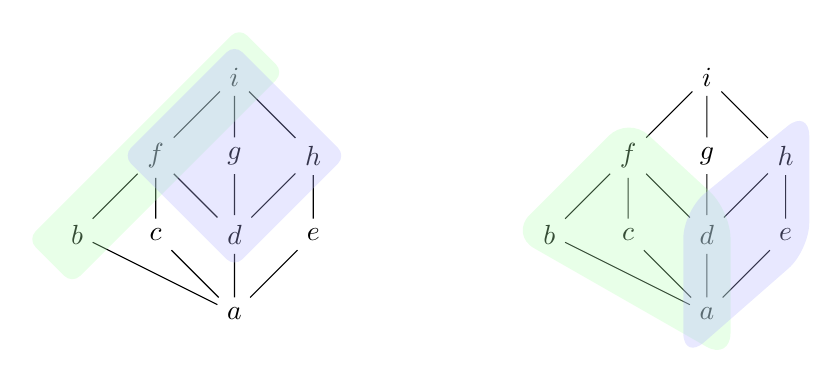
\begin{tikzpicture}
    \begin{scope}
        \node (a) at (2,0) {$a$};
        \node (b) at (0,1) {$b$};
        \node (c) at (1,1) {$c$};
        \node (d) at (2,1) {$d$};
        \node (e) at (3,1) {$e$};
        \node (f) at (1,2) {$f$};
        \node (g) at (2,2) {$g$};
        \node (h) at (3,2) {$h$};
        \node (i) at (2,3) {$i$};
        \draw (a)--(b)--(f)--(c)--(a)--(d)--(f)--(i)--(g)--(d)--(a)--(e)--(h)--(i); \draw (h)--(d);

        \node[fill=green!30, opacity=0.3, rectangle, rounded corners, rotate=45, minimum width=3.8cm, minimum height=.8cm] at (1,2){};
        \node[fill=blue!30, opacity=0.3, rectangle, rounded corners, rotate=45, minimum width=2cm, minimum height=2cm] at (2,2){};
    \end{scope}
    \begin{scope}[xshift=6cm]
        \node (a) at (2,0) {$a$};
        \node (b) at (0,1) {$b$};
        \node (c) at (1,1) {$c$};
        \node (d) at (2,1) {$d$};
        \node (e) at (3,1) {$e$};
        \node (f) at (1,2) {$f$};
        \node (g) at (2,2) {$g$};
        \node (h) at (3,2) {$h$};
        \node (i) at (2,3) {$i$};
        \draw (a)--(b)--(f)--(c)--(a)--(d)--(f)--(i)--(g)--(d)--(a)--(e)--(h)--(i); \draw (h)--(d);


        \fill[rounded corners=10pt, fill=green!30, opacity=0.3] (-.5,1) -- (1,2.5) -- (2.3,1.3) -- (2.3,-.6) -- cycle;
        \fill[rounded corners=10pt, fill=blue!30, opacity=0.3] (1.7,-.6) -- (1.7,1.3) -- (3.3,2.6) -- (3.3,.8) -- cycle;
    \end{scope}
    \end{tikzpicture}
    \caption{束上のフィルター(左)とイデアル(右)の例.それぞれ緑色・青色の枠で囲った部分はフィルター/イデアルになっている.}
    \label{fig:filter} 
\end{figure}

\begin{renshu}{}{}
図\ref{fig:filter}を参考に,上のもの以外の固有フィルターと固有イデアルを一つづつあげよ.
\end{renshu}

フィルターとイデアルの「ご利益」は一見してあまり明らかではないかもしれないが,様々なところに出てくる概念である.
例えば我々は事例\ref{rei:truthfunction}で,準同型写像$f:L' \to \bbB$が論理式集合$L'$上の真理値関数となることを見た.
この逆像$f^{-1}(\texttt{true})$はフィルターであり,$f^{-1}(\texttt{false})$はイデアルとなる.
しかも両者には明確な意味がある:前者は関数$f$のもとで真となる論理式全体であり,後者は偽となる論理式全体である.

% fca: intent and extent
% \begin{rei}{概念の内包}{}
% 再び概念の束を考えよう.
% 個々の概念$c \in C$は,「人間である」「哺乳類である」といった属性であるともいえる.
% この見方のもとで,ある概念は,それより上位のすべての概念およびその連言概念を属性としてすべて含む,といえる.例えば人間であれば,二足歩行であり,哺乳類であり,動物であり,かつ「哺乳類かつ二足歩行」でもあり,云々.
% このように,ある概念が持つ全属性を,その概念の\emph{内包}(intent)と呼ぶ.
% 内包はフィルターである.
% \end{rei}

\begin{rei}{概念を用いた推論}{}
我々は日常,観察した対象の性質からそれが何であるかを同定し,そこからさらなる性質を引き出すことによって推論を行う.
例えば目の前の物体が「硬い$H$」「光沢がある$S$」ということから,それが「金属$M$」であると同定し,それによってその物体は金属に一般的な他の性質,例えば「導電性$C$」なども持つと推論する\footnote{もちろん,ニクロムやアルマイトなど電気抵抗が高い金属が存在するので,こうした推論はあくまで蓋然的なものに過ぎないが,ここではその点は無視する.}.
フィルターを用いることで,こうした推論をモデル化できる(図\ref{fig:inference}).
その推論過程としては,まず対象$x$が$Hx \wedge Sx$であることから,その交わり$Mx$でもあることが帰結される.
次に$x$は$M$の例化として,$M$の内包,すなわちそのフィルターに含まれる性質全てを持つことが導かる.
導電性$C$は$M$の内包に含まれる性質であるため,$Cx$が帰結する.
つまり,対象を同定するとは,その対象にとって既知の性質$H, S$のフィルターを取ることに想定し,それによってそのフィルターに含まれる未観測の性質$C$をその対象に帰属させることができるのである.
\end{rei}

\begin{figure}[h]
    \centering
    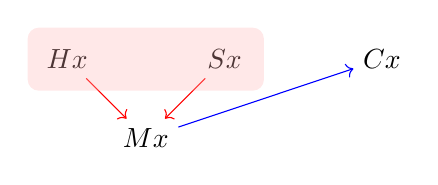
\begin{tikzpicture}
        \node (h) at (0,2) {$Hx$};
        \node (s) at (2,2) {$Sx$};
        \node (m) at (1,1) {$Mx$};
        \node (c) at (4,2) {$Cx$};

        \draw[->, red] (h)--(m);
        \draw[->, red] (s)--(m);
        \draw[->, blue] (m)--(c);
        \node[fill=red!30, opacity=0.3, rectangle, rounded corners, minimum width=3cm, minimum height=.8cm] at (1,2){};
        % \node[fill=blue!30, opacity=0.3, rectangle, rounded corners, rotate=45, minimum width=2cm, minimum height=2cm] at (2,2){};
    \end{tikzpicture}
    \caption{フィルターを用いた推論.赤で囲まれた観測された事実$Hx, Sx$を証拠として,$x$がその結び$M$であることがまず帰結される(赤矢印).次に,それが$M$の内包すなわちフィルターに含まれる他の性質,例えば$C$を持つことが結論される(青矢印).}
    \label{fig:inference} 
\end{figure}



%\begin{develop}
%上の事例は,個々の概念をその内包と同一視する可能性を示唆している.
%\end{develop}

図\ref{fig:filter}でも明らかなように,同じ束の中に様々なフィルターが存在する.
さらにこれらの間には大小がある.
例えばフィルター$F = \{i,g\}$は$F' = \{i, f, g, h, d\}$にすっぽり収まるので,$F \subset F'$となっている.
このとき,$F$と$F'$は比較可能であり,$F$はより荒い/$F'$はより細かいという\footnote{これは束上のフィルターの集合が半順序になっていることを示唆する.それは束だろうか?どんな束だろうか?}.
すべてのフィルターが比較可能であるわけではない.例えば$F'' = \{i, f, b\}$は$F$より細かいが,$F'$とは比較可能ではない.

束全体$X$は当然すべてのフィルターよりも細かいが,それを除外して,比較可能なすべての固有フィルターよりも細かいような固有フィルターを,\emph{超フィルター}(ultra filter)と呼ぶ.
上の$F', F''$はそれぞれ超フィルターである.
ここから明らかなように,超フィルターは一つとは限らず,複数ありえる.
超フィルターは,それよりも何かを一つでも足してフィルターを作ろうとすると,束全体となって固有フィルターではなくなってしまう,そのようなフィルターである.
例えば$F'$に$b$を足してできるフィルターは,$d \wedge b = a$を含むので,最小元より上のすべて,つまり束全体を含んでしまうことになる.

% 粗さ・細かさの定義は全く同様の仕方でイデアルに対しても適用される.
% そして,比較可能なすべての固有イデアルよりも細かい固有イデアルは,\emph{最大イデアル}(maximal ideal)と呼ばれる.

\begin{renshu}{}{}
    図\ref{fig:filter}上の超フィルターをすべて挙げよ.
\end{renshu}

\begin{rei}{科学理論と予測の詳細さ}{theory}
科学理論$T$は現実世界について何らかの予測を立てる.
ここから理論$T$を$T$によって予測されるすべての命題の集合と同一視しよう.
この集合は当然,帰結関係と連言に関して閉じているだろう,つまりある理論$T$が「来週いっぱい晴れである」と予測するなら,そこから帰結する「来週月曜は晴れである」とも予測するだろうし,またさらに「来週の最高気温は30度である」と予測するなら,「来週いっぱいは晴れで最高気温は30度である」も予測するはずだ.
よって理論は,命題束上の固有フィルターとして考えることができる.
より詳細な予測をする理論ほど,良い理論といえる.
「来週月曜は晴れである」と予測する理論より,「来週月曜日は晴れで最高気温は30度である」と予測する理論のほうがより「細かく」世界のあり方を規定している.
この解釈では,フィルターの細かさは,対応する科学理論の予測の詳細さに対応している.
(ではこの解釈において,超フィルターは何を表すだろうか.)
\end{rei}



\section{ブール代数}

束は2つの二項演算$\vee$と$\wedge$を持ち,これは当然論理演算の「または」と「かつ」に対応していることを上の事例を通して確認してきた.
しかし気がついたと思うが,そこでは周到に「否定を除く」という但し書きをつけてきた.
というのも否定というのは2項ではなく1項演算$\neg:p \mapsto \neg p$であり,単なる束の中には対応物が無いからである.
この否定演算を加え,さらに$\vee$と$\wedge$についての分配則を付け加えたものを,\emph{ブール代数}(Boolean algebra)と呼ぶ.

\begin{dfn}{ブール代数}{bool}
    最大元1と最小元0を持つ束$\langle X, \preceq \rangle$が以下を満たすとき,ブール代数と呼ばれる
    \begin{enumerate}
        \item \emph{分配則}(distributive law)を満たす,つまりすべての$x, y, z \in X$に対し,
        \begin{align}
         x \wedge (y \vee z) = (x \wedge y) \vee (x \wedge z) \label{eqn:dist1}\\
         x \vee (y \wedge z) = (x \vee y) \wedge (x \vee z) . \label{eqn:dist2}
        \end{align}
        \item 否定演算$\neg: X \to X, x \mapsto \neg x$があり,次の\emph{排中律}(law of excluded middle)を満たす
        \begin{equation}
            x \vee \neg x = 1, \ \ \ x \wedge \neg x = 0
           \label{eqn:excluded_middle}
        \end{equation}
        なお$\neg x$を$x$の補元(complement)と呼ぶ.
    \end{enumerate}   
\end{dfn}

分配則(\ref{eqn:dist1}), (\ref{eqn:dist2})については1章の集合演算のところで見覚えがあるだろう.また結びと交わりを$+$と$\times$に置き換えれば,これは小学校で習った分配則と全く同じ形をしている\footnote{実際この類似性は偶然ではなく,圏論的な観点からいえば,これらはみな余積(co-product)および積(product)という一般的な構造の例である.}.
分配束とは,これら2つの演算がどうやって組み合わさるのか,ということを表す法則である.

一方,否定$\neg$はここで登場した新しい演算子である.
これは束の中の一つの元$x \in X$をとって,これを元$\neg x \in X$に対応させる1項関数である.
排中律は,このようにしてできる$x, \neg x$の関係性を規定している.
外見から明らかなように,これは明らかに古典論理の否定に対応している.
実際(\ref{eqn:excluded_middle})は,「$p$または$\neg p$」は常に真$\top$,「$p$かつ$\neg p$」は常に偽$\bot$という論理学の排中律・矛盾律そのままである.

% Theorems in boolean alg
%このおかげで,ブール代数ではド・モルガン則のもう一方が成立する
%\begin{equation}
% \neg (x \wedge y) = \neg x \vee \neg y.
%\end{equation}

図\ref{fig:8bool}は,8元からなるブール代数(左側)と,ブール代数ではない束(右側)を示している.
右側の束では,排中律を満たすような否定演算を定義することはできるが,分配束が満たされない.
実際,$\neg a = b, \neg c = e, \neg d =f, \neg 0 = 1$のようにとれば,これらのペアの結びは$1$,交わりは$0$となり排中律を満たす(ただし,その取り方は一意ではない.例えば$\neg c = f$のようにしても同様に成り立つ).
一方,例えば$a \vee (d \wedge e) = a \vee 0 = a$であるが,$(a \vee d) \wedge (a \vee e) = d \wedge 1 = d$となり,両者は一致しない.
よってこれはブール代数ではない.
\begin{figure}[h]
    \centering
    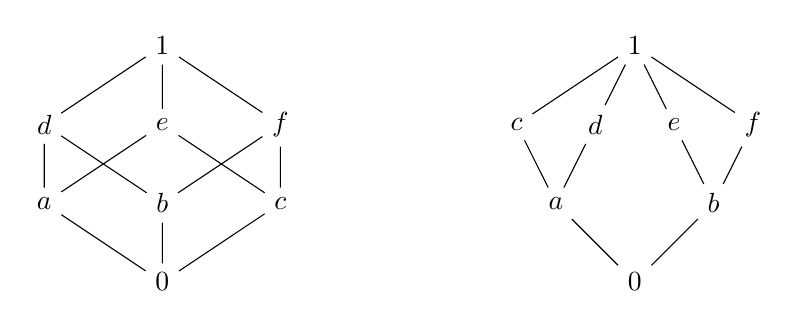
\begin{tikzpicture}[node distance=1.5cm]
        \begin{scope}
        \node (0) at (0,0) {$0$};
        \node (11) at (-1.5,1) {$a$};
        \node (12) at (0,1) {$b$};
        \node (13) at (1.5,1) {$c$};
        \node (21) at (-1.5,2) {$d$};
        \node (22) at (0,2) {$e$};
        \node (23) at (1.5,2) {$f$};
        \node (1) at (0,3) {$1$};      
        % Now you need to draw the lines between the nodes
        \draw (0)--(11)--(21)--(1)--(23)--(13)--(0);
        \draw (0)--(12)--(21); \draw (12)--(23);
        \draw (1)--(22)--(11); \draw (22)--(13);
        \end{scope} 
        \begin{scope}[xshift=6cm]
        \node (0) at (0,0) {$0$};
        \node (11) at (-1,1) {$a$};
        \node (12) at (1,1) {$b$};
        \node (21) at (-1.5,2) {$c$};
        \node (22) at (-0.5,2) {$d$};
        \node (23) at (0.5,2) {$e$};
        \node (24) at (1.5,2) {$f$};
        \node (1) at (0,3) {$1$};      
        % Now you need to draw the lines between the nodes
        \draw (0)--(11)--(21)--(1)--(22)--(11);
        \draw (0)--(12)--(23)--(1)--(24)--(12);
        \end{scope} 
    \end{tikzpicture}
    \caption{8元からなるブール代数(左)とそうでない束(右).}
    \label{fig:8bool}
\end{figure}

\begin{renshu}{}{}
 図\ref{fig:8bool}左において,
 \begin{enumerate}
  \item (1) $d \wedge (e \vee f)$, (2) $a \vee (b \wedge c)$, (3) $e \wedge (d \vee f)$ をそれぞれ計算せよ.
  \item (1) $(d \wedge e) \vee (d \wedge f)$, (2) $(a \vee b) \wedge (a \vee c)$, (3) $(e \wedge d) \vee (e \wedge f)$ をそれぞれ計算せよ.
  \item $\neg a, \neg b, \neg c$を求めよ.
 \end{enumerate}
\end{renshu}


我々は2節で,束について複数の定理(1)-(5)が成立することを見た.
ブール代数では分配束と排中律が加えられたことにより,さらに多くの定理が成立する.代表的なものを少し挙げておこう.
\begin{align}
\neg 0 = 1 &, \ \ \ \neg 1 = 0  \\
\neg \neg x &= x \\
\neg (x \vee y) &= \neg x \wedge \neg y \\
\neg (x \wedge y) &= \neg x \vee \neg y
\end{align}
特に(10)は二重否定除去,(11-12)はド・モルガン則と呼ばれる.


\begin{figure}[h]
    \centering
    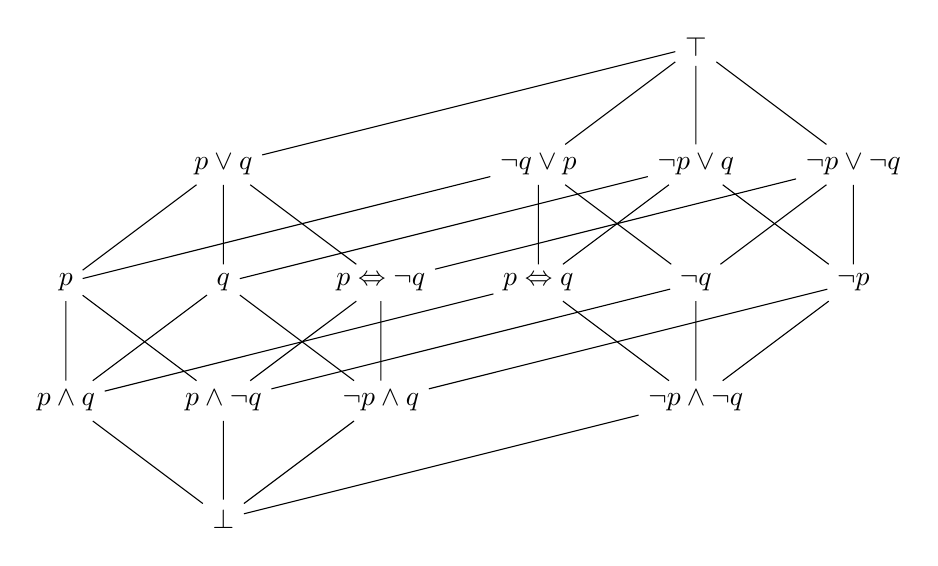
\begin{tikzpicture}[node distance=1.5cm]
        \node (0) at (-1,0) {$\bot$};
        % 1st layer
        \node (11) at (-3,1.5) {$p \wedge q$};
        \node (12) at (-1,1.5) {$p \wedge \neg q$};
        \node (13) at (1,1.5) {$\neg p \wedge q$};
        \node (14) at (5,1.5) {$\neg p \wedge \neg q$};
        % 2nd layer
        \node (21) at (-3,3) {$p$};
        \node (22) at (-1,3) {$q$};
        \node (23) at (3,3) {$p \Leftrightarrow q$};
        \node (24) at (1,3) {$p \Leftrightarrow \neg q$};
        \node (25) at (5,3) {$\neg q$};
        \node (26) at (7,3) {$\neg p$};
        % 3rd layer
        \node (31) at (-1,4.5) {$p \vee q$};
        \node (32) at (3,4.5) {$\neg q \vee p$};
        \node (33) at (5,4.5) {$\neg p \vee q$};
        \node (34) at (7,4.5) {$\neg p \vee \neg q$};
        % top layer
        \node (1) at (5,6) {$\top$};
      
        % Now you need to draw the lines between the nodes
        \draw (11)--(0)--(12)--(0)--(13)--(0)--(14);
        \draw (11)--(21)--(12);
        \draw (11)--(22)--(13);
        \draw (11)--(23)--(14);
        \draw (12)--(24)--(13);
        \draw (12)--(25)--(14);
        \draw (13)--(26)--(14);
        \draw (31)--(21)--(32);
        \draw (31)--(22)--(33);
        \draw (32)--(23)--(33);
        \draw (31)--(24)--(34);
        \draw (32)--(25)--(34);
        \draw (33)--(26)--(34);
        \draw (31)--(1)--(32)--(1)--(33)--(1)--(34);
    \end{tikzpicture}
    \caption{単純命題$p, q$から構成される命題論理のブール代数のハッセ図.左右の立方体は,それぞれの否定を含んでいる.}
    \label{fig:bool}
\end{figure}

\begin{rei}{}{}
    命題論理の束$\langle L', \vdash \rangle$は,ブール代数である.
    2つの単純命題$p, q$のみからなるブール代数$L'$は,図\ref{fig:bool}のようになる.見方によっては,2つの立方体の頂点間が結ばれたように見える.ここにおいて,上で見たブール代数の公理が成立していることを確認してみよう.

    まず,分配則の一つ目$x \wedge (y \vee z) = (x \wedge y) \vee (x \wedge z) $をみる.いま,$x = p, y = p \iff q, z = \neg p$ととってみる.
    左辺から見ると,$p \iff q$と$\neg p$の結びは$\neg p \vee q$,それと$p$の交わりは$p \wedge q$になる.
    次に右辺を見ると,$p$と$p \iff q$の交わりは$p \wedge q$であり,$p$と$\neg p$の交わりは$\bot$.よってそれらの結びは$p \wedge q$となり,確かに両辺は一致している.
    
    次に否定の例も見てみよう.$p \wedge q$を例にとると,その否定は$\neg p \vee \neg q$である.両者の上側の合流点つまり結びは$\top$であり,下側の合流点つまり交わりは$\bot$であるので,排中律(\ref{eqn:excluded_middle})が成立している.
    ちなみにこの図では,一方の立方体に属する元の否定が他方の立方体の,それもちょうど対称的な頂点に位置していることに注意せよ.
    これ以外にも適当な元を選んで,上の公理が成立していることを確認してみよう.
\end{rei}

\begin{renshu}{}{}
 \begin{enumerate}
    \item 2値順序$\bbB = \{ \texttt{false, true} \}$は,ブール代数である.それぞれの補元は何か.
    \item $X = \{a, b, c\}$として,ブール代数$\langle \mcalP(X), \subset \rangle$のハッセ図を書け.任意の元$A \in \mcalP(X)$の補元は何か.また分配束・排中律が満たされることを確認せよ.
 \end{enumerate}
\end{renshu}

束を用いたモデリングにおいて,否定は必ずとも存在するとは限らない.
例えば事例\ref{rei:mereology}で見たメレオロジーにおいて,一般にその束の要素は「個物」であると解釈されている(つまりメレオロジーとは個物の間の部分全体関係を扱うものである).
そう考えたとき,ある個物の「否定」が何であるかは必ずしも明らかではない.
例えば「エッフェル塔の否定」とはなんだろうか.それはエッフェル塔以外のすべての「部分」と言って良いのか.そうだとして,それは「個物」なのだろうか.
もしこれが否であるなら,メレオロジー束をブール代数として扱うことは適当ではない.


\begin{rei}{スコトゥスと「正反対のモノ」}{scotus}
 ドゥンス・スコトゥスは以下のような議論をしたといわれている\footnote{マレンボン『哲学がわかる 中世哲学』(周藤多紀訳,岩波書店, p. 108)}. ある具体的な黒いモノ,例えばこの黒猫に正反対なものを考えてみよ.少なくともそれは白いものでなければならないが,しかし白いものはいくらでもあるので,そうした反対物が一意に定まることはない.よって個物の「反対物」を実在するものとして考えることはできない.
 これは,概念の束(事例\ref{rei:concept})では,少なくともそれが具体的な個体を含む限り,否定が定義できず,よってブール代数ではない,という議論だと解釈できる.
\end{rei}

\begin{renshu}{}{}
    \begin{enumerate}
        \item では,具体的な個体を含まないような概念の束は,ブール代数たりえるだろうか.
        \item 可能世界の束(事例\ref{rei:p-worlds})はブール代数だろうか.
    \end{enumerate}
\end{renshu}



\subsection{ブール代数上のフィルター}

我々は前節でフィルターとイデアルの概念を見た.
さらに超フィルターを,最も細かい(つまり比較可能な固有フィルターをすべて含む)フィルターとして定義した.
ブール代数は束なので,当然そこにもこれらはそのままの定義で妥当する.
さらにブール代数では,超フィルターは「すべての元につき,それかその否定のどちらかが含まれている」フィルターとしても定義できる.つまり次が成り立つ.
\begin{prop}{}{}
    \begin{quote}
        $F$がブール代数$B$上の超フィルターである 
        \\ $\iff$ すべての$x \in B$について,$x \in F$あるいは$\neg x \in F$.    
    \end{quote}
\end{prop}

これは命題論理のブール代数$\langle L', \vdash \rangle$を例に取れば,超フィルターとはすべての式についてその式かその否定のどちらかが含まれている論理式の集合だといえる.
我々は後に,これが命題論理の真理値割当に一致することを確認する.

\begin{renshu}{}{}
    図\ref{fig:bool}において,
    \begin{enumerate}
        \item $p \iff q$を含む最小のフィルターおよびイデアルは何か.
        \item $p$および$p \iff q$を含む最小のフィルターは何か.
        \item このブール代数からは何個の異なる超フィルターを取れるか.
    \end{enumerate}
\end{renshu}

\begin{rei}{完全な理論}{}
事例\ref{rei:theory}で,科学理論を命題論理の束上のフィルターと同一視した.
この解釈では,超フィルターとは,すべての事態$p$について,その肯定か否定が理論によって予測されるような,完全な理論であるといえる.
\end{rei}    

\begin{rei}{汎通的規定}{}
概念の束(事例\ref{rei:concept})がブール代数をなすと仮定しよう.
これはつまり,あらゆる概念につきその否定概念,例えば「赤い」という概念に対し「赤くない」も概念だと認めるということだ.
この概念の束における超フィルターとは,すべての概念につき,その肯定か否定かどちらかが必ず含まれるようなものである.
カントはこれを汎通的規定と呼んだ.
そしてカントによれば,個体とは全ての概念について汎通的に規定されているものである:つまり我々は,すべての概念について,それが属するか属さないかを完全に(汎通的に)定めることで,個体概念にたどり着くのである.
よって概念束$C$がすべての概念を含むという仮定のもとで,個体とは$C$上の超フィルターである.
\end{rei}

\begin{rei}{反証可能性}{}
    再び事例\ref{rei:theory}の科学理論フィルターを考える.
    このフィルターを部分として含む全命題はブール代数$X$を構成するとする.
    ポパーによれば,理論$T$はその予測に反する観測が得られたとき,反証される.
    $T$を反証する観測の集合を反証集合$I(T)$とすると,$I(T)=\{ x \in X | \exists t \in T (x = \neg t) \}$である.
    これは$X$上のイデアルとなる(確認せよ).
    また,$T \subset T'$であれば,$I(T) \subset I(T')$である(確認せよ).
    よって理論が細かくより詳細な予測を行うほど,より反証集合が大きく,反証されるリスクが高いといえる.
    一方ポパーによれば,疑似科学とは決して反証できない理論,すなわち$I(T_0)= \{ \emptyset \}$であるような理論$T_0$である.
    この予測集合は$T_0 = \{1\}$となる,つまり疑似科学は何の具体的予測も行わない.
\end{rei}
% boolean homomorphism

\subsection{ブール準同型}

最後にブール代数間の準同型写像を,以下のように定義する.

\begin{dfn}{ブール準同型}{bool_homomorphism}
    ブール代数$X, Y$間の束準同型$f:X \to Y$が,さらに以下の条件を満たすとき,\emph{ブール準同型}(Boolean homomorphism)と呼ぶ:
    \[ \text{すべての } x \in X \text{ について, } f(\neg x) = \neg f(x) . \]
\end{dfn}

つまりブール準同型は,束準同型として順序,結び,交わりを保存するだけでなく,さらに最大/最小元および否定を保存するような写像である.
実際,これらがブール代数を構成するすべてのアイテムなので,これらを保存する写像は,確かにブール代数の構造をしっかりと写し取っているといえる.
また以前と同様,$f$が全単射であるとき,ブール同型写像であるといわれる.

\begin{prop}{}{}
    ブール準同型写像$f:X \to Y$は最大元および最小元を保存する,つまり$f(1_X)=1_Y$ かつ $f(0_X) = 0_Y$が成り立つ.(ただし$1_X, 1_Y$は$X$および$Y$の最大元,$0_X, 0_Y$は最小元). 最大元だけ示すと:
    \begin{align*}
        f(1_X) &= f (x \vee \neg x)   
        & \because & \ (\ref{eqn:excluded_middle}) \\
        &= f (x) \vee f(\neg x) 
        & \because & \ f \text{は束準同型} \\
        &= f (x) \vee \neg f(x) 
        & \because & \ f \text{はブール準同型} \\
        &= 1. 
        & \because & \ (\ref{eqn:excluded_middle})
    \end{align*}
\end{prop}

\begin{rei}{}{}
命題論理ブール代数$\langle L', \vdash \rangle$から2値順序$\bbB = \{ \true, \false \}$への準同型写像は,真理値関数にほかならない.
条件$f( \neg p) = \neg f(p)$は否定演算子の真理値表に対応していることを確認せよ.
また任意の真理値関数$f$について,$F = f^{-1}(\true)$はそのもとで真になる論理式全体である.
このとき,任意の$p \in L$について,$f(p)=\true$ならば逆像の定義より$p \in F$であり,$f(p)=\false$であれば否定の保存条件より$f(\neg p) = \neg f(p) = \neg \false = \true$となるため,$\neg p \in F$である.
つまり$F = f^{-1}(\true)$は超フィルターである.
\end{rei}

\begin{rei}{}{}
    事例\ref{rei:p-worlds}で見た命題から可能世界の集合への写像は,ブール準同型になる.
    また\ref{rei:extension}で見た概念からその外延への写像も,概念束がブール代数になるという仮定のもとでブール準同型となる.
\end{rei}

% 我々はこれまで,ブール代数の重要な事例としてべき集合系$\langle \mcalP(X), \subset \rangle$を見てきた.
% これは「$x$は$y$\emph{に含まれる}」を意味する「$\subset$」で順序付けられているので,上(最大元1)に近づくほど大きな集合になる.
% しかし今,この関係を逆転させて,「$x$は$y$\emph{を含む}」を意味する$\supset$で順序付けてみると,実はこれもちゃんとしたブール代数になる.
% ただしそこでの「最大元」(あらゆる集合に含まれる)は空集合$\empty$であり,「最小元」は$X$である.
% また$\vee, \wedge$もそれぞれ$\cup, \cap$と逆になる.
% 一般に,あらゆる順序/束/ブール代数はこのように順序を逆転させても順序/束/ブール代数になる.
% 順序/束/ブール代数$X$をそっくり反転させたものを$X^{op}$と書く.つまり
% \[ \langle \mcalP(X), \subset, \cup, \cap, 1, 0, ^C \rangle^{op}
% = \langle \mcalP(X), \supset, \cap, \cup, 0, 1, ^C \rangle  \]
% である.

% こうした反転を考える利点は,次の事例から明らかになる.

% \begin{rei}
% 命題論理ブール代数$\langle L', \vdash \rangle$および可能世界の集合$W$を考える.
% 関数$f:L' \to W$を, 命題$p \in L'$に対しそれが成立している世界の集合$f(p) \subset W$を対応させる関数とする.
% すると$f$は$L'$から$\mcalP(W)^{op}$へのブール準同型写像となる.
% \end{rei}


\subsection{ブール代数の表現*}

最後に発展的な話題を少し.我々はこれまで,任意のブール代数(命題,概念,等々)はべき集合のブール代数(可能世界の集合,外延の集合,等々)と密接に関連していることを見てきた.
これは偶然ではない.実際のところ,あらゆるブール代数はなんらかのべき集合と同一視できる---つまり任意のブール代数について,それと同型のべき集合代数があり,またべき集合代数があれば,それとブール同型なブール代数を作ることができる.
\emph{ストーンの表現定理}(Stone's representation theorem)として知られるこの結果は,統語論的構造(ブール代数)と意味論的構造(集合族)の結びつきを示すものとして非常に重要である.
任意のブール代数についてこれを示すのは大変だが,有限の場合であれば比較的簡単なので,以下に素描しよう.

まず$B$を有限ブール代数とする.$B$の元$a$で,最小元$0$スレスレのもの,すなわち$0 \preceq a, a \neq 0$だが$a$未満のものは$0$しかない,そんな元を$B$の\emph{原子}(atom)と呼ぶ(視覚的には原子は最小元の「直上の層」にくる:図\ref{fig:atoms}参照).
$B$のすべての原子の集合を$\mcalA(B)$で表そう.
すると$B$の任意の元$b \in B$は,その下にある原子の和になることが示せる,つまり
\[ b = \bigvee \{ x \in \mcalA(B) | x \preceq b \}. \]
このことは,図\ref{fig:atoms}でも確認できる(図ではこれを明示するため,元自体をその下にある構成原子によって示している).

ここまで来たら,あとは任意の$b \in B$をその「素材」となる原子の集合に飛ばす写像$\eta$を考えればよい
\[ \eta: b \mapsto \{ x \in \mcalA(B) | x \preceq b \} \]
この写像は$B$からアトム集合のべき集合$\mcalP(\mcalA(B))$へのブール同型になっている.
逆写像は,任意のアトム集合$S \subset \mcalA(B)$に対しその和としてのブール元を返す$\eta^{-1}: S \mapsto \bigvee S$である.
このようにして,任意の有限ブール代数はべき集合として表現できることがわかった.


\begin{figure}[h]
    \centering
    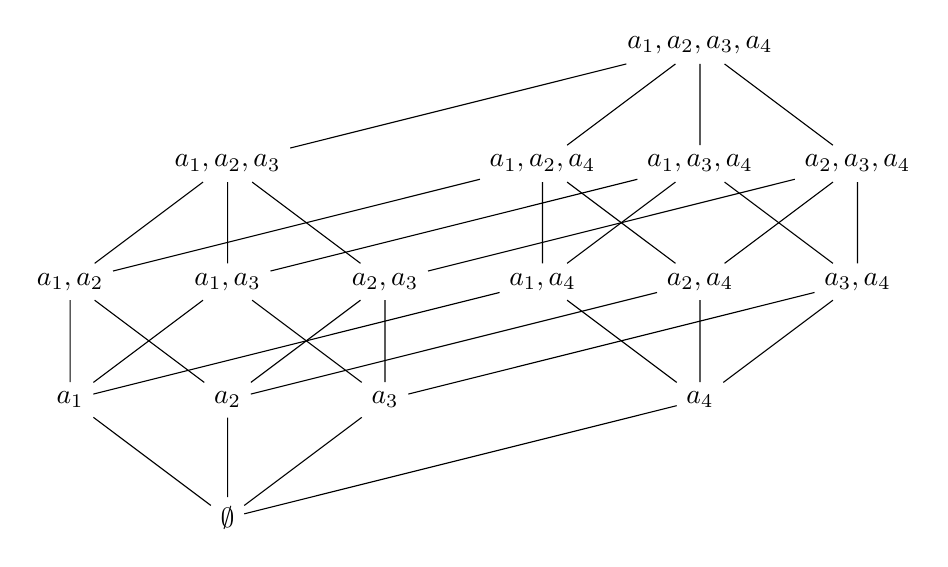
\begin{tikzpicture}[node distance=1.5cm]
        \node (0) at (-1,0) {$\emptyset$};
        % 1st layer
        \node (11) at (-3,1.5) {$a_1$};
        \node (12) at (-1,1.5) {$a_2$};
        \node (13) at (1,1.5) {$a_3$};
        \node (14) at (5,1.5) {$a_4$};
        % 2nd layer
        \node (21) at (-3,3) {$a_1, a_2$};
        \node (22) at (-1,3) {$a_1, a_3$};
        \node (23) at (3,3)  {$a_1, a_4$};
        \node (24) at (1,3) {$a_2, a_3$};
        \node (25) at (5,3) {$a_2, a_4$};
        \node (26) at (7,3) {$a_3, a_4$};
        % 3rd layer
        \node (31) at (-1,4.5) {$a_1, a_2, a_3$};
        \node (32) at (3,4.5)  {$a_1, a_2, a_4$};
        \node (33) at (5,4.5) {$a_1, a_3, a_4$};
        \node (34) at (7,4.5) {$a_2, a_3, a_4$};
        % top layer
        \node (1) at (5,6) {$a_1, a_2, a_3, a_4$};
      
        % Now you need to draw the lines between the nodes
        \draw (11)--(0)--(12)--(0)--(13)--(0)--(14);
        \draw (11)--(21)--(12);
        \draw (11)--(22)--(13);
        \draw (11)--(23)--(14);
        \draw (12)--(24)--(13);
        \draw (12)--(25)--(14);
        \draw (13)--(26)--(14);
        \draw (31)--(21)--(32);
        \draw (31)--(22)--(33);
        \draw (32)--(23)--(33);
        \draw (31)--(24)--(34);
        \draw (32)--(25)--(34);
        \draw (33)--(26)--(34);
        \draw (31)--(1)--(32)--(1)--(33)--(1)--(34);
    \end{tikzpicture}
    \caption{図\ref{fig:bool}と同じ16元ブール代数の構成.原子集合$\mcalA(B) = \{a_1, a_2, a_3, a_4\}$である.すべての元が原子集合の部分集合として表せていることを確認しよう.}
    \label{fig:atoms} 
\end{figure}


%問題\ref{q:logic}と\ref{q:set}は,命題論理の理論と部分集合の体系が,ブール代数として見ると同じ構造を持っている,ということを(非常にシンプルなケースで)示している.
% しばしばいわれるように,命題論理というのは記号の間に成り立つ統語論的な関係であり,集合はその意味論を与える(例えば命題$P$に対して$P$が成り立つ可能世界の集合が対応する).
% するとこの対応は,統語論(論理)と意味論(集合)との対応だといえる.
% では,こうした関係は一般に成り立つのだろうか.
% 答えはYesであって,任意の命題論理の体系は,何らかの集合の体系と一対一に対応する,ということが証明できる.
% しかしそのためには,どのような集合の体系であれば命題論理との体系と対応するのか,ということを定める必要がある(というのも,明らかに任意の集合を命題論理の意味論を与えるものとして解釈することはできないからだ).
% 具体的には,そのためには位相構造(次章参照)を集合に入れてやる必要がある.
% その上で,命題論理の体系は,そうした特定の位相構造を持つ集合の系,具体的には\emph{ストーン空間}(stone space)と呼ばれる位相空間と同型であることが示せる.
% この命題論理の統語論と意味論を結びつける結果は,\emph{ストーンの表現定理}(Stone's representation theorem)と呼ばれている.
% これは非常に重要な定理であり,あとで扱う位相や圏論とも関連が深いのだが,この授業内では扱うことができない.
% 関心がある向きは,Hans Halvorson, \textit{The Logic in Philosophy of Science}などを参照されたい(ただし結構むずかしい).



% \section{ハイティング代数}

% 有限束にさらに公理を加えて,パワーアップさせてみよう.

% \begin{dfn}[ハイティング代数]
% (有限)\emph{ハイティング代数}(Heyting algebra)とは,0と1を持つ束 $\langle X, \preceq \rangle$であり,かつ結びと交わりが以下の\emph{分配則}(distributive law)を満たすものである:すべての$x, y, z \in X$に対し,
% \begin{align}
%  x \wedge (y \vee z) = (x \wedge y) \vee (x \wedge z) \\
%  x \vee (y \wedge z) = (x \vee y) \wedge (x \vee z) .
% \end{align}
% \end{dfn}

% 結びと交わりを$+$と$\times$に置き換えれば,これは小学校で習った分配則と全く同じ形をしている\footnote{実際,圏論的な観点からいえば,結びと足し算は余積(co-product),交わりと掛け算は積(product)という一般的な構造の例である.}.
% ハイティング代数とは,この分配則が成り立つ完備束である.

% ハイティングは直観論理(intuitionistic logic)で知られるオランダの数学者.
% 実際,ハイティング代数は直観論理(排中律が成り立たない)のモデルとして提唱された.
% また後の章で見るように,位相空間とも密接に対応している.

% 上で,束には2つの演算$\vee, \wedge$が備わっていることを見た.
% ハイティング代数では更に,\emph{含意}(implication)と呼ばれる次の演算$\Rightarrow$が定義できる.
% \[
%  z \preceq (x \Rightarrow y) \iff z \wedge x \preceq y
% \]
% これはどう読めばよいのだろう.
% まず左辺は,$x, y$という2つの元に「含意」演算を施して得られる元$x \Rightarrow y$が他のある元$z$よりも上にある,という事態を表している.
% そして右辺と合わせた条件式全体は,こうした事態が成立するのは,$z \wedge x$が$y$より下にあるとき,そのときのみであるということをいっている.
% このようにしてこの式は,「含意」演算を施して得られた元$x \Rightarrow y$が束上で占める位置を右辺によって定めることにより,演算を定義している.

% 具体的には,$x \Rightarrow y$は$z \wedge x \preceq y$を満たすような$z$たちの上限になっている.
% $y$自身は$y \wedge x \preceq y$を満たすので,$y \preceq (x \Rightarrow y)$,つまり$x \Rightarrow y$は$y$の上にある.
% しかし同時に,$x \Rightarrow y$と$x$の交わりは$y$より下,つまり$(x \Rightarrow y) \wedge x = y \wedge x$でなければならない.
% $x \Rightarrow y$はそのような条件を満たす元の中で一番上にある元である.

% \begin{rei}
% 含意の定義はややこしい.しかし論理学を知っていると少しそのややこしさは和らぐかもしれない.
% その名前から推察されるように,含意$x \Rightarrow y$は命題論理における実質含意を念頭においている.
% そしてその記号から推察されるように,結び$\vee$と交わり$\wedge$はそれぞれ「または」と「かつ」に対応している.
% では順序$\preceq$は何に対応しているかというと,帰結関係$\vdash$である.
% 例えば$x \wedge y \preceq z$は,$x \wedge y \vdash z$,つまり$x$かつ$y$なら$x$が成り立つ,という論理的真理を表している(同様のことを$\vee$でも確かめよ).
% これを念頭に上で定義した含意を論理式に翻訳すると,
% \[
%  z \vdash (x \Rightarrow y) \iff z \wedge x \vdash y
% \]
% となる.これは,$z$から「$x$ならば$y$」が帰結するならば,「$z$かつ$x$」から$y$が帰結するし,また逆もしかり,という\emph{演繹定理}(deduction theorem)を表している.
% こう考えると,上で述べたように$x \Rightarrow y$が$y$の上にあるのも納得できるし($y$が成り立っていれば$x \Rightarrow y$は必ず成り立つ),$(x \Rightarrow y) \wedge x = y \wedge x$も真理表から確認できる.
% \end{rei}


% さて,ハイティング代数には$0$があるので,任意の$x \in X$について$x \Rightarrow 0$が存在する.
% これを\emph{擬補元}(pseudo-complement)と呼び,$\neg x$で表す.
% これは$x$をとって$x \Rightarrow 0$を返す演算
% \[
%  \neg:: x \mapsto \neg x = x \Rightarrow 0
% \]
% と考えることもできる.

% ハイティング代数で新たに加わった演算についても,様々な定理が成立する.
% 例えば$\Rightarrow$については
% \begin{align}
%  x \Rightarrow x &= 1 \\
% ((x \wedge (x \Rightarrow y)) \Rightarrow y) &= 1 \label{eqn:md}\\
% (x \vee y ) \Rightarrow z &= (x \Rightarrow z) \vee (y \Rightarrow z) \\
% x \Rightarrow (y \wedge z ) &= (x \Rightarrow y) \wedge (x \Rightarrow z) 
% \end{align}
% などが任意の$x, y, z \in X$について成立する.また$\neg$に関しては
% \begin{align}
%  x & \preceq \neg \neg x \\
%  \neg (x \vee y) &= \neg x \wedge \neg y
% \end{align}
% などが成立する.

% \begin{rei}
% 上述したように,ハイティング代数は直観主義論理のモデルを与える.
% それを見るには,$\vee, \wedge, \Rightarrow, \neg$をそれぞれ論理和(または),論理積(かつ),実質含意(ならば),否定(〜でない)に読み替え,各元を命題記号と考えれば良い.
% この観点からは,例えば(8)と(9)はそれぞれ同一律およびmodus ponensが常にトートロジーであること,(10)と(11)は「ならば」の分配則に対応していることがわかる.
% 一方(13)はド・モルガン法の一方を示す(もう片方はすぐ後で見るブール代数のみで成り立つ).
% また(12)において,$x$の二重否定が$x$と一致しないのにも注意せよ.これは直観主義論理において二重否定が除去できないことに対応する.
% \end{rei}




% \begin{develop}
% ここでの取り扱いはすべて有限束を前提としている.
% 無限束の場合は,ハイティング代数であるためには完備性と\emph{無限分配束}を満たさなければならない.
% 前節で触れたように,完備性とは任意の(無限でも良い)部分集合に上限と下限が存在すること.
% そして無限分配則とは,任意の(無限でも良い)部分集合$Y \subset X$について,$x \wedge (\bigvee_{y \in Y} y) = \bigvee_{y \in Y}(x \wedge y)$が成立する(交わりも同様)ことである.
% 完備性のときと同様,無限束においては,分配則が満たされていても無限分配則は満たされないことがありうる.

% こうした無限・有限の区別を避けるために,教科書によっては,ハイティング代数を「任意の2元が含意を持つ完備束」と定義することもある.
% その場合,(無限)分配則はそこからの定理として導かれる.
% いずれにせよ,両流儀の定義は一致する.
% \end{develop}



\end{document}